

Signals are often thought of as the product of sources that act statistically.
Our goal is to model these statistical properties. Our basis of model building depends on 
assumptions about liminations in the model's degree of freedom. 
Further the model should deliver useful information for segmenting signals into meaningful units
\cite{mm_pr}[p.71]

A \emph{Hidden Markov Model} describe a \textbf{two-state stochastic process}.
There is a stochastic process that is stationary (which means its probabilistic features don't change over time) and a \emph{state space} that is finite.
A \emph{Markov Chain Model} probabilistically describes the state transitions as a \emph{finite state automaton} - see table \ref{tab:FiniteSA}.

% figure for state transition table as finite state automaton
\begin{table}[h]
	\begin{center}
		\begin{tabular}{| c | c |}
			\hline
			\multicolumn{2}{|l|}{
				\begin{tabular}{ l }
					\emph{Finite state automatons} \\
				\end{tabular}
			} \\
			\hline
			& \\
			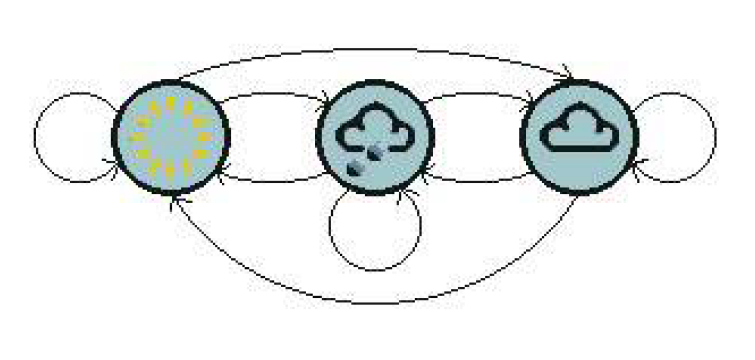
\includegraphics[width=0.33\textwidth]{./Images/FiniteStateAutomaton_1.png} & 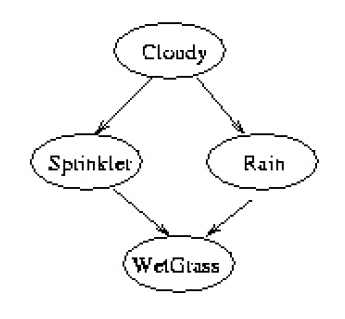
\includegraphics[width=0.33\textwidth]{./Images/FiniteStateAutomaton_2.png} \\
			\hline
			weather HMM \cite{hmm_fb} & grass HMM \cite{gm_bn} \\
			\hline
		\end{tabular}
	\end{center}
	\caption{Two finite state automatons that describe the state space of two different HMMs. Nodes correspond to states and edges to transition probabilites betwenn states that are bigger than $0$.}
	\label{tab:FiniteSA}
\end{table}

The important thing is that \textbf{the behaviour of the process given at time $t$ only depends on the immedate predessor state}. So the \emph{Markov property} \eqref{eq:markProp} states:

\begin{equation}
	P(S_t | S_1,S_2, \ldots S_{t-1}) = P(S_t | S_{t-1})
	\label{eq:markProp}
\end{equation}

Visually this can be shown with a graph model of a HMM as a sequence of hidden states $X_i$ and the corresponding obervations $Y_i$ - see figure \ref{fig:GraphModel}.

% GraphModelHMM_1.png
\begin{figure}[H]
	\centering
	
	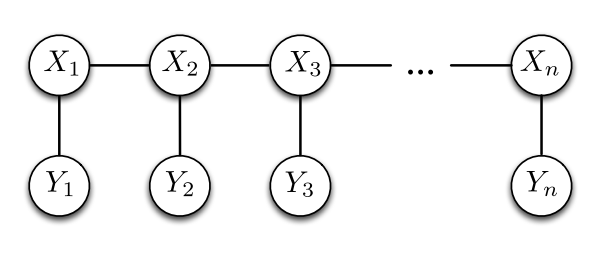
\includegraphics[width=0.66\textwidth]{./Images/GraphModelHMM_1.png}
	\caption{ \cite{hmm_II}}
	\label{fig:GraphModel}
\end{figure}

In the second stage at every point in time $t$ an output obervation $O_t$ (or $Y_t$) is generated. The corresponding \textbf{probability distribution only depend on the current state}. This is called the \emph{output independence assumption} \eqref{eq:outIndep}.

\begin{equation}
P(O_t | O_1,O_2, \ldots O_{t-1}) = P(O_t | S_{t-1})
\label{eq:outIndep}
\end{equation} 

The model itself is \emph{'hidden'} because we only can observe the outputs generated, namely the \emph{observation sequence} $O_1, O_2, \ldots,  O_T$.

For initialization of the model additional start probalilities are used that describe the start probability distribution at time $t=1$.

A hidden Markov model denoted as $\lambda$ is described by \cite{mm_pr}[p.73]:

\begin{itemize}
	\item a finite set of states $S$ \\ 
	$ S = \left\{s | 1 \leq s \leq N \right\} $
	\item a state-transition probalilitiy matrix $A$ \\ 
	$A = \left\{ a_{ij} | a_{ij} = P(S_t = j | S_{t-1} = i) \right\}$
	\item a start probability vector $\Pi$ \\ 
	$ \Pi = \left\{ \Pi_i | \Pi_i = P(S_1 = i)  \right\}$
	\item specific state probability dirstibutions for the outputs of the model,  \\
	$\left\{ b_j(o_k) | b_j(o_k) = P(O_t = o_k | S_t = j) \right\}$ \\
	if observations are discrete we can write in matrix form \\
	$ B = \left\{ b_{kj} | b_{kj} = P(O_t = o_k | S_t = j) \right\} $
\end{itemize}